\documentclass[fleqn,10pt]{wlscirep}
\usepackage[utf8]{inputenc}
\usepackage[T1]{fontenc}
\usepackage{lineno}
\usepackage{float}
\linenumbers

\usepackage{color}
\usepackage{fancyvrb}
\newcommand{\VerbBar}{|}
\newcommand{\VERB}{\Verb[commandchars=\\\{\}]}
\DefineVerbatimEnvironment{Highlighting}{Verbatim}{commandchars=\\\{\}}
% Add ',fontsize=\small' for more characters per line
\usepackage{framed}
\definecolor{shadecolor}{RGB}{248,248,248}
\newenvironment{Shaded}{\begin{snugshade}}{\end{snugshade}}
\newcommand{\AlertTok}[1]{\textcolor[rgb]{0.94,0.16,0.16}{#1}}
\newcommand{\AnnotationTok}[1]{\textcolor[rgb]{0.56,0.35,0.01}{\textbf{\textit{#1}}}}
\newcommand{\AttributeTok}[1]{\textcolor[rgb]{0.77,0.63,0.00}{#1}}
\newcommand{\BaseNTok}[1]{\textcolor[rgb]{0.00,0.00,0.81}{#1}}
\newcommand{\BuiltInTok}[1]{#1}
\newcommand{\CharTok}[1]{\textcolor[rgb]{0.31,0.60,0.02}{#1}}
\newcommand{\CommentTok}[1]{\textcolor[rgb]{0.56,0.35,0.01}{\textit{#1}}}
\newcommand{\CommentVarTok}[1]{\textcolor[rgb]{0.56,0.35,0.01}{\textbf{\textit{#1}}}}
\newcommand{\ConstantTok}[1]{\textcolor[rgb]{0.00,0.00,0.00}{#1}}
\newcommand{\ControlFlowTok}[1]{\textcolor[rgb]{0.13,0.29,0.53}{\textbf{#1}}}
\newcommand{\DataTypeTok}[1]{\textcolor[rgb]{0.13,0.29,0.53}{#1}}
\newcommand{\DecValTok}[1]{\textcolor[rgb]{0.00,0.00,0.81}{#1}}
\newcommand{\DocumentationTok}[1]{\textcolor[rgb]{0.56,0.35,0.01}{\textbf{\textit{#1}}}}
\newcommand{\ErrorTok}[1]{\textcolor[rgb]{0.64,0.00,0.00}{\textbf{#1}}}
\newcommand{\ExtensionTok}[1]{#1}
\newcommand{\FloatTok}[1]{\textcolor[rgb]{0.00,0.00,0.81}{#1}}
\newcommand{\FunctionTok}[1]{\textcolor[rgb]{0.00,0.00,0.00}{#1}}
\newcommand{\ImportTok}[1]{#1}
\newcommand{\InformationTok}[1]{\textcolor[rgb]{0.56,0.35,0.01}{\textbf{\textit{#1}}}}
\newcommand{\KeywordTok}[1]{\textcolor[rgb]{0.13,0.29,0.53}{\textbf{#1}}}
\newcommand{\NormalTok}[1]{#1}
\newcommand{\OperatorTok}[1]{\textcolor[rgb]{0.81,0.36,0.00}{\textbf{#1}}}
\newcommand{\OtherTok}[1]{\textcolor[rgb]{0.56,0.35,0.01}{#1}}
\newcommand{\PreprocessorTok}[1]{\textcolor[rgb]{0.56,0.35,0.01}{\textit{#1}}}
\newcommand{\RegionMarkerTok}[1]{#1}
\newcommand{\SpecialCharTok}[1]{\textcolor[rgb]{0.00,0.00,0.00}{#1}}
\newcommand{\SpecialStringTok}[1]{\textcolor[rgb]{0.31,0.60,0.02}{#1}}
\newcommand{\StringTok}[1]{\textcolor[rgb]{0.31,0.60,0.02}{#1}}
\newcommand{\VariableTok}[1]{\textcolor[rgb]{0.00,0.00,0.00}{#1}}
\newcommand{\VerbatimStringTok}[1]{\textcolor[rgb]{0.31,0.60,0.02}{#1}}
\newcommand{\WarningTok}[1]{\textcolor[rgb]{0.56,0.35,0.01}{\textbf{\textit{#1}}}}

\newlength{\cslhangindent}
\setlength{\cslhangindent}{1.5em}
\newenvironment{CSLReferences}%
{\setlength{\parindent}{0pt}%
\everypar{\setlength{\hangindent}{\cslhangindent}}\ignorespaces}%
{\par}

\title{Multiorder Hydrologic Position in Europe as a Set of Metrics in Support of Groundwater Mapping at Regional and National Scales}

\author[*, 1]{Maximilian Nölscher}
\author[2]{Michael Mutz}
\author[1]{Stefan Broda}
\affil[1]{Federal Institute for Geosciences and Natural Resources (BGR), Sub-Department: Basic information Groundwater and Soil (B2.2), Berlin, 13593, Germany}
\affil[2]{independet researcher}
\affil[*]{corresponding author: Maximilian Nölscher (max-n@posteo.de)}


\begin{abstract}
This dataset (EU-MOHP v013.0.1) provides information on the multiorder hydrologic position of a geographic point within its respective river network or catchment. More precisely, it comprises the three measures ``lateral position'' as a relative measure of the position between the stream and the catchment boundary/ watershed, ``divide stream distance'' as an absolute distance measure that serves as a proxy for the position within the catchment and ``stream distance'' as an absolute measure of the distance to the nearest stream. These three measures were calculated for several hydrologic (stream) orders. Its spatial extent covers major parts of physiographical Europe and all of the 39 countries in European Economic Area (EEA39). Although there might be many potential use cases, this dataset serves predominantly as valuable input data for mapping tasks in the context of hydrogeology and subsurface characteristics in general. \cite{belitz_multiorder_2019}
\end{abstract}
\begin{document}

\flushbottom
\maketitle
%  Click the title above to edit the author information and abstract

\thispagestyle{empty}

\hypertarget{background-summary}{%
\section{Background \& Summary}\label{background-summary}}

In recent years, data science tools such as machine learning are increasingly applied to and specifically developed for hydro(geo)logical challenges and research questions. In the field of hydrogeology, machine learning has been used successfully for groundwater level prediction and a variety of mapping tasks. Since machine learning models are traditionally based purely on data with no built-in knowledge of physical processes, it is important to provide as many variables (predictor variables/ explanatory variables/ features) as possible that have an impact on the target variable to potentially enable the machine learning algorithm to reproduce the result of the underlying process. For surface and near-surface processes, this criterion may be more or less satisfiable through the availability of remote sensing data, whereas for modelling subsurface processes such as in hydrogeology, this poses a serious challenge. \cite{desimone_machine-learning_2020, belitz_multiorder_2019}

\begin{Shaded}
\begin{Highlighting}[]
\NormalTok{asd }\OtherTok{\textless{}{-}} \StringTok{"sdf"}
\end{Highlighting}
\end{Shaded}

\hypertarget{methods}{%
\section*{Methods}\label{methods}}
\addcontentsline{toc}{section}{Methods}

Text.
\ref{fig:flowchart}

\hypertarget{data-records}{%
\section*{Data Records}\label{data-records}}
\addcontentsline{toc}{section}{Data Records}

Text.

\hypertarget{technical-validation}{%
\section*{Technical Validation}\label{technical-validation}}
\addcontentsline{toc}{section}{Technical Validation}

Text.

\hypertarget{usage-notes}{%
\section*{Usage Notes}\label{usage-notes}}
\addcontentsline{toc}{section}{Usage Notes}

Text.

\hypertarget{code-availability}{%
\section*{Code availability}\label{code-availability}}
\addcontentsline{toc}{section}{Code availability}

Text.

\hypertarget{acknowledgements}{%
\section*{Acknowledgements}\label{acknowledgements}}
\addcontentsline{toc}{section}{Acknowledgements}

Text.

\hypertarget{author-contributions-statement}{%
\section*{Author contributions statement}\label{author-contributions-statement}}
\addcontentsline{toc}{section}{Author contributions statement}

Text.

\hypertarget{competing-interests}{%
\section*{Competing interests}\label{competing-interests}}
\addcontentsline{toc}{section}{Competing interests}

Text.

\hypertarget{figures-tables}{%
\section*{Figures \& Tables}\label{figures-tables}}
\addcontentsline{toc}{section}{Figures \& Tables}

\begin{figure}

{\centering 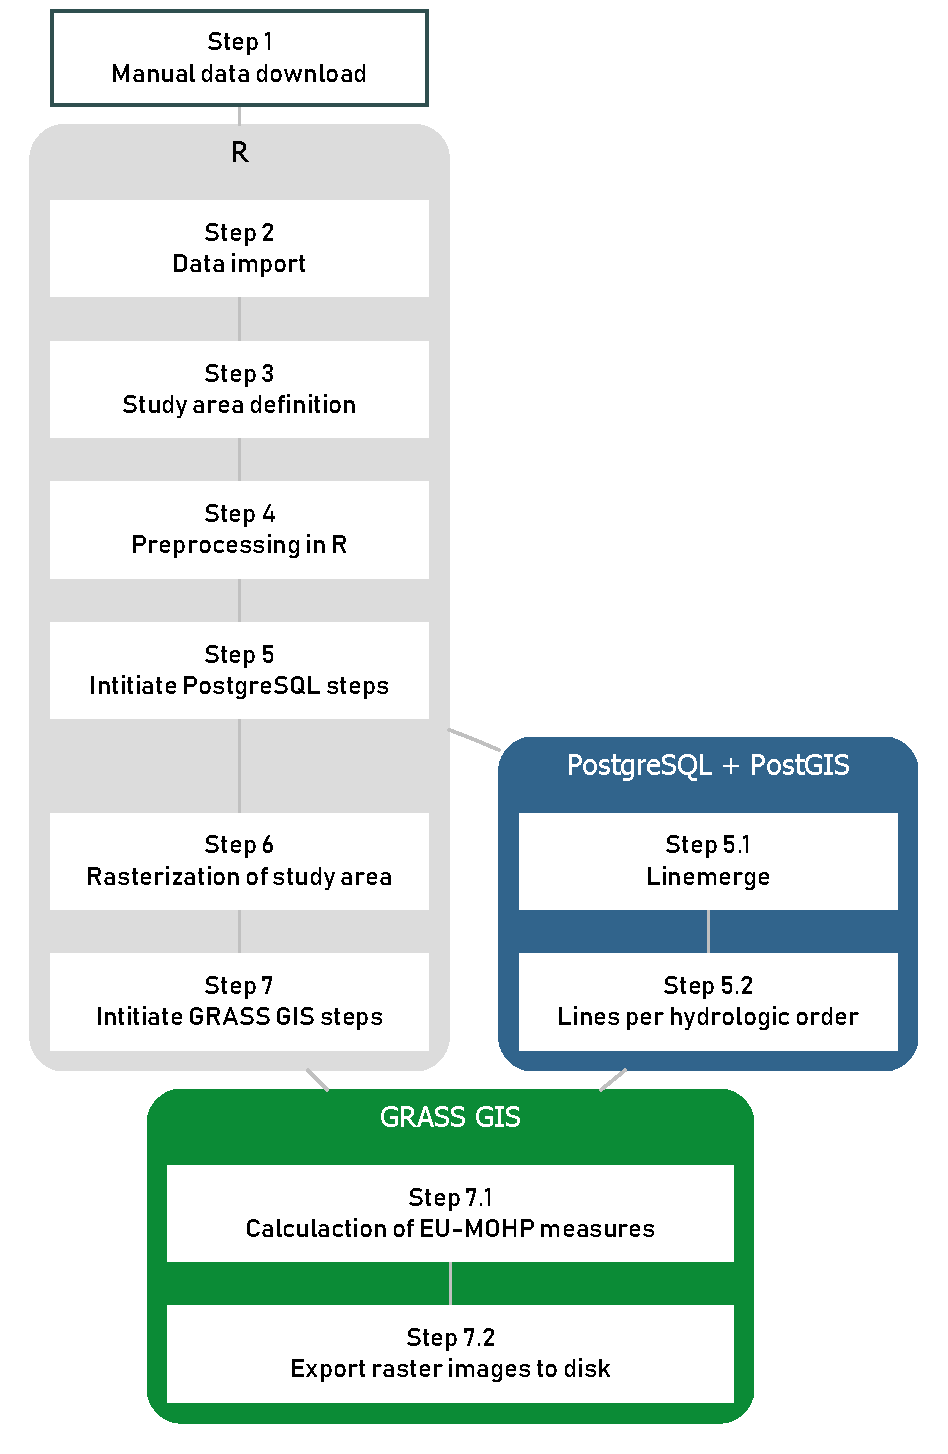
\includegraphics[width=0.7\linewidth]{diagramms/flowchart} 

}

\caption{sdf}\label{fig:flowchart}
\end{figure}

\bibliography{eumohp.bib}

\end{document}
